\section{Supplementary Figures}
 \begin{figure}[!ht]
    \centering
     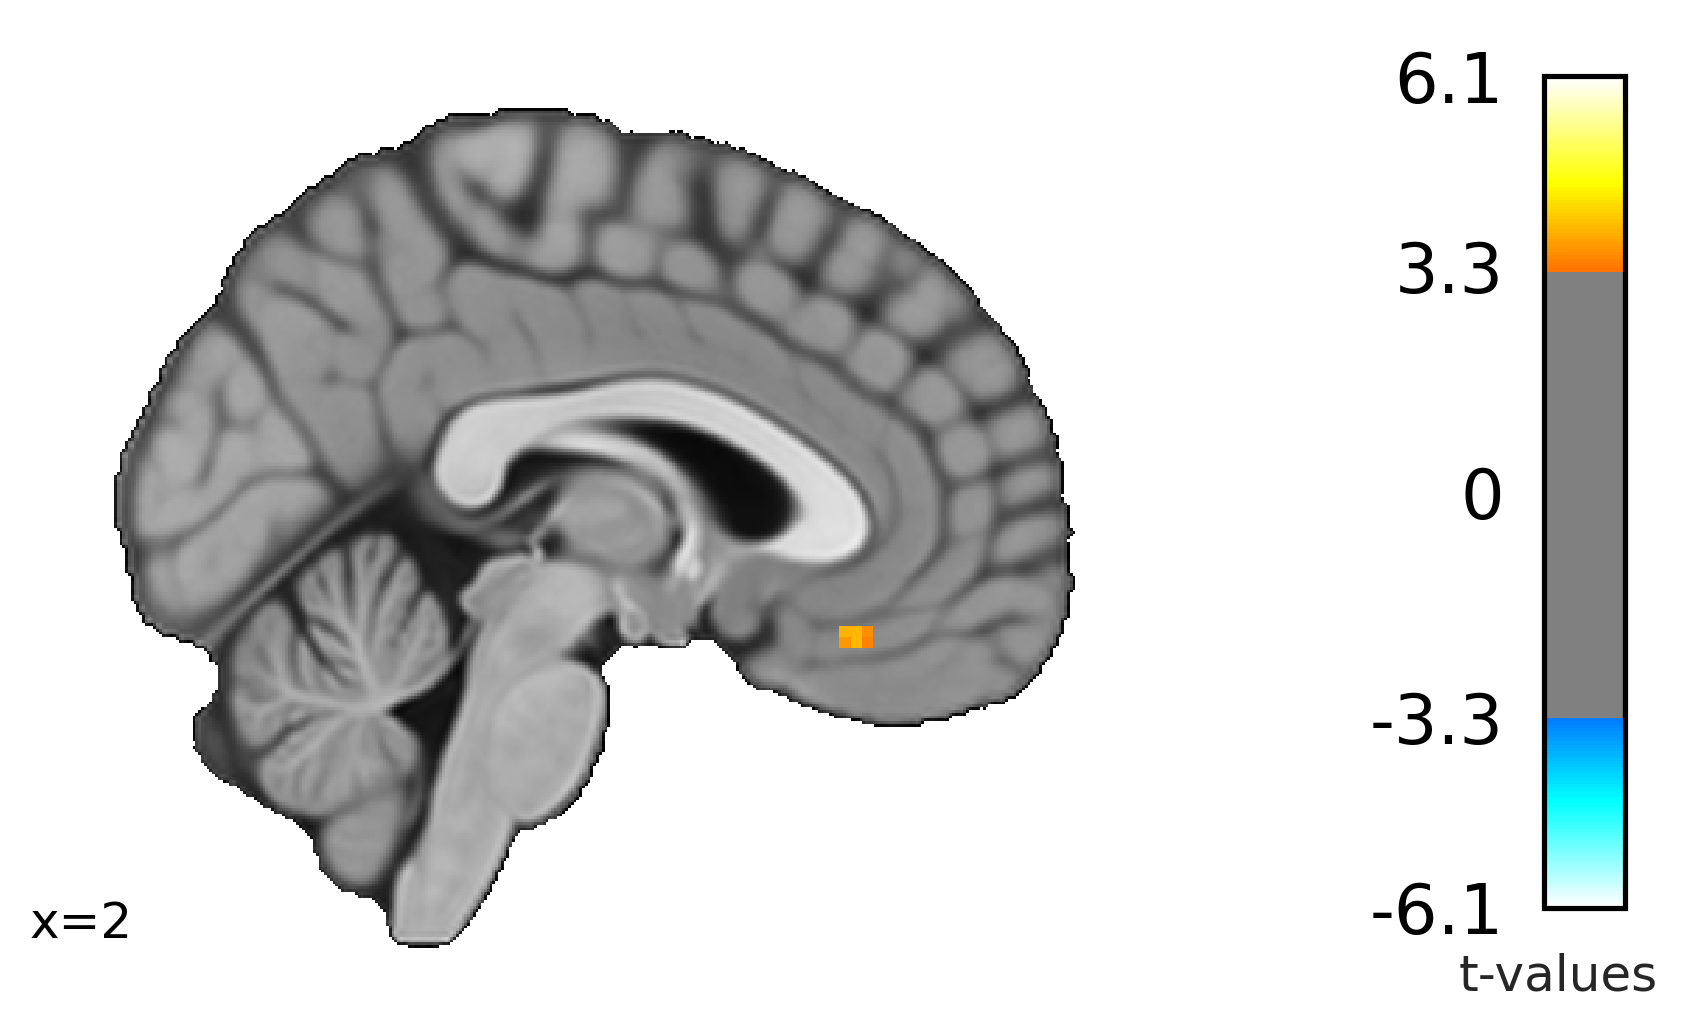
\includegraphics[width=\linewidth/2]{paper/src/figures/FigureS1_inaccessible_subsequent.png}
     \caption*{\textbf{Figure S1. Medial prefrontal cortex activation during guess responses given at the 24-hour category retrieval predicted the subsequent regain of conscious access to the memories.} \\ \vspace{0.5em}
     Medial prefrontal component of the episodic retrieval network predicted conscious recognition success. We contrasted the guess responses on the 24-hour category retrieval task that would subsequently yield correct sure responses on the recognition task with those other guess responses given on the 24-hour category task that would subsequently yield correct guess responses on the recognition task. This revealed a cluster in the medial prefrontal cortex (peak at MNI [0, 30, -16], p\textsubscript{uncor} < 0.001, T(18) = 4.19). Results presented in this panel were acquired with the whole-brain fMRI sequence. See Table S12 for details.}
\end{figure}

\newpage


 \begin{figure}[!ht]
    \centering
\begin{subfigure}[]{0.6\linewidth}
    \centering
    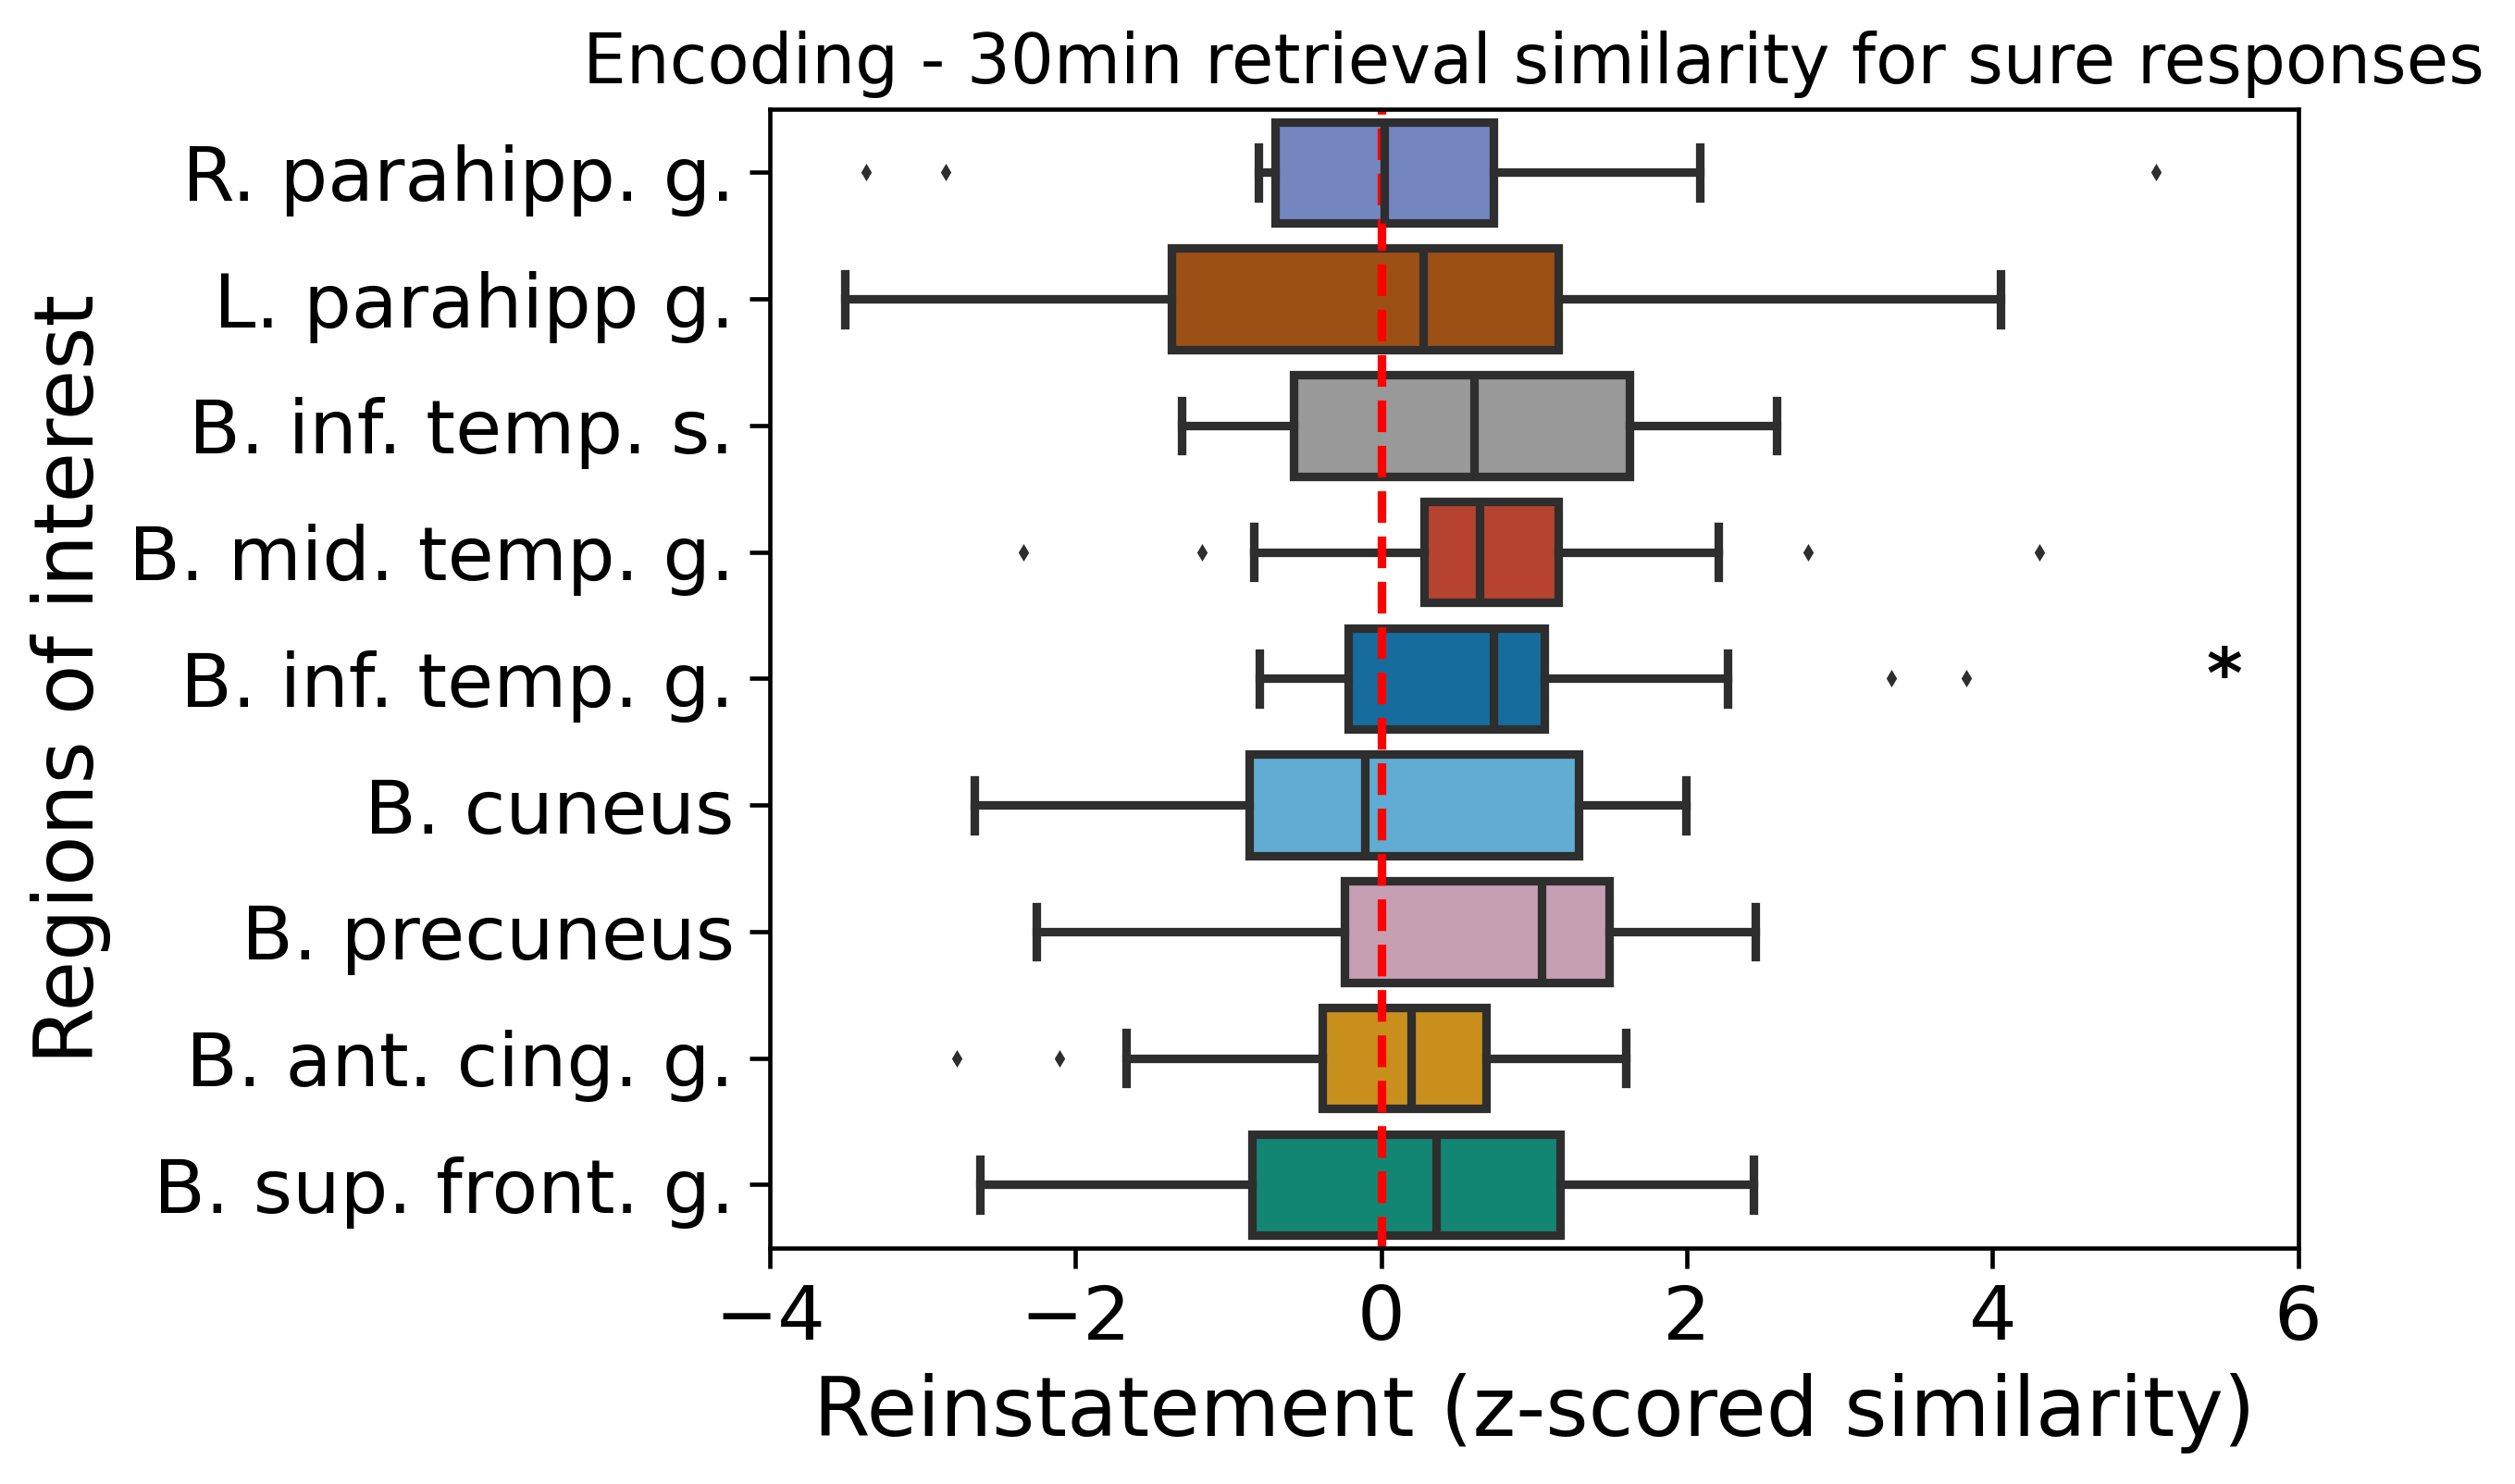
\includegraphics[width=\linewidth]{paper/src/figures/20240530_wb-array_n__enc_ret1_perm_consc_consc-unconsc_incorr.png}
\end{subfigure}
\begin{subfigure}[]{0.19\linewidth}
    \centering
    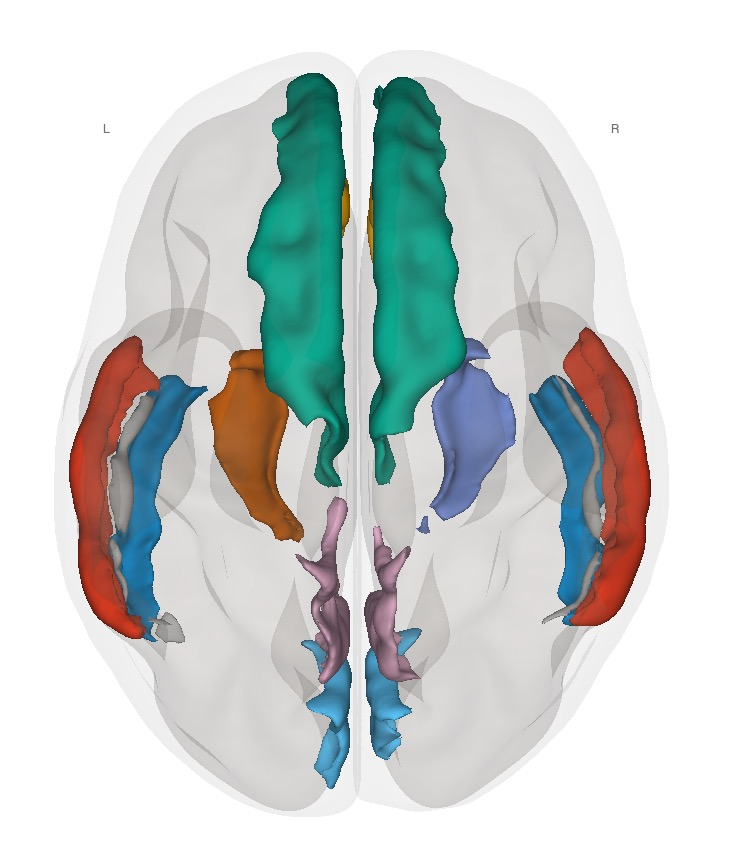
\includegraphics[width=\linewidth]{paper/src/figures/wb_rois_top.jpg}
\end{subfigure}
\begin{subfigure}[]{0.19\linewidth}
    \centering
    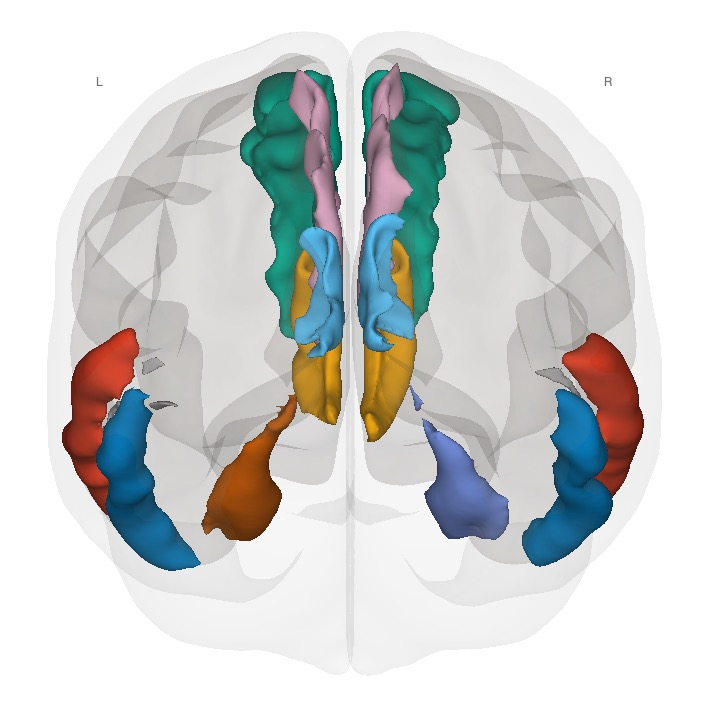
\includegraphics[width=\linewidth]{paper/src/figures/wb_rois_back.jpg}
\end{subfigure}
     \caption*{\textbf{Figure S2. Similarity of voxel patterns between encoding and the 30-minute category retrieval task was relevant for retrieval accuracy.} \\ \vspace{0.5em}
Encoding – retrieval similarity (ERS) analysis for the 30-minute category retrieval yielded significance in the bilateral inferior temporal gyrus for correct sure responses (t(16) = 2.3, p = 0.035, B\textsubscript{10} = 1.9).  Results presented in this panel were acquired with the whole-brain fMRI sequence. *p < 0.05, **p < 0.01 by Student’s t test. Abbreviations: R., right; L., left; B., bilateral; parahipp., parahippocampus; inf., inferior; mid., middle; ant., anterior; cing., cingulate; sup., superior; front., frontal; s., sulcus, g., gyrus.
}
\end{figure}

\newpage


 \begin{figure}[!ht]
    \centering
     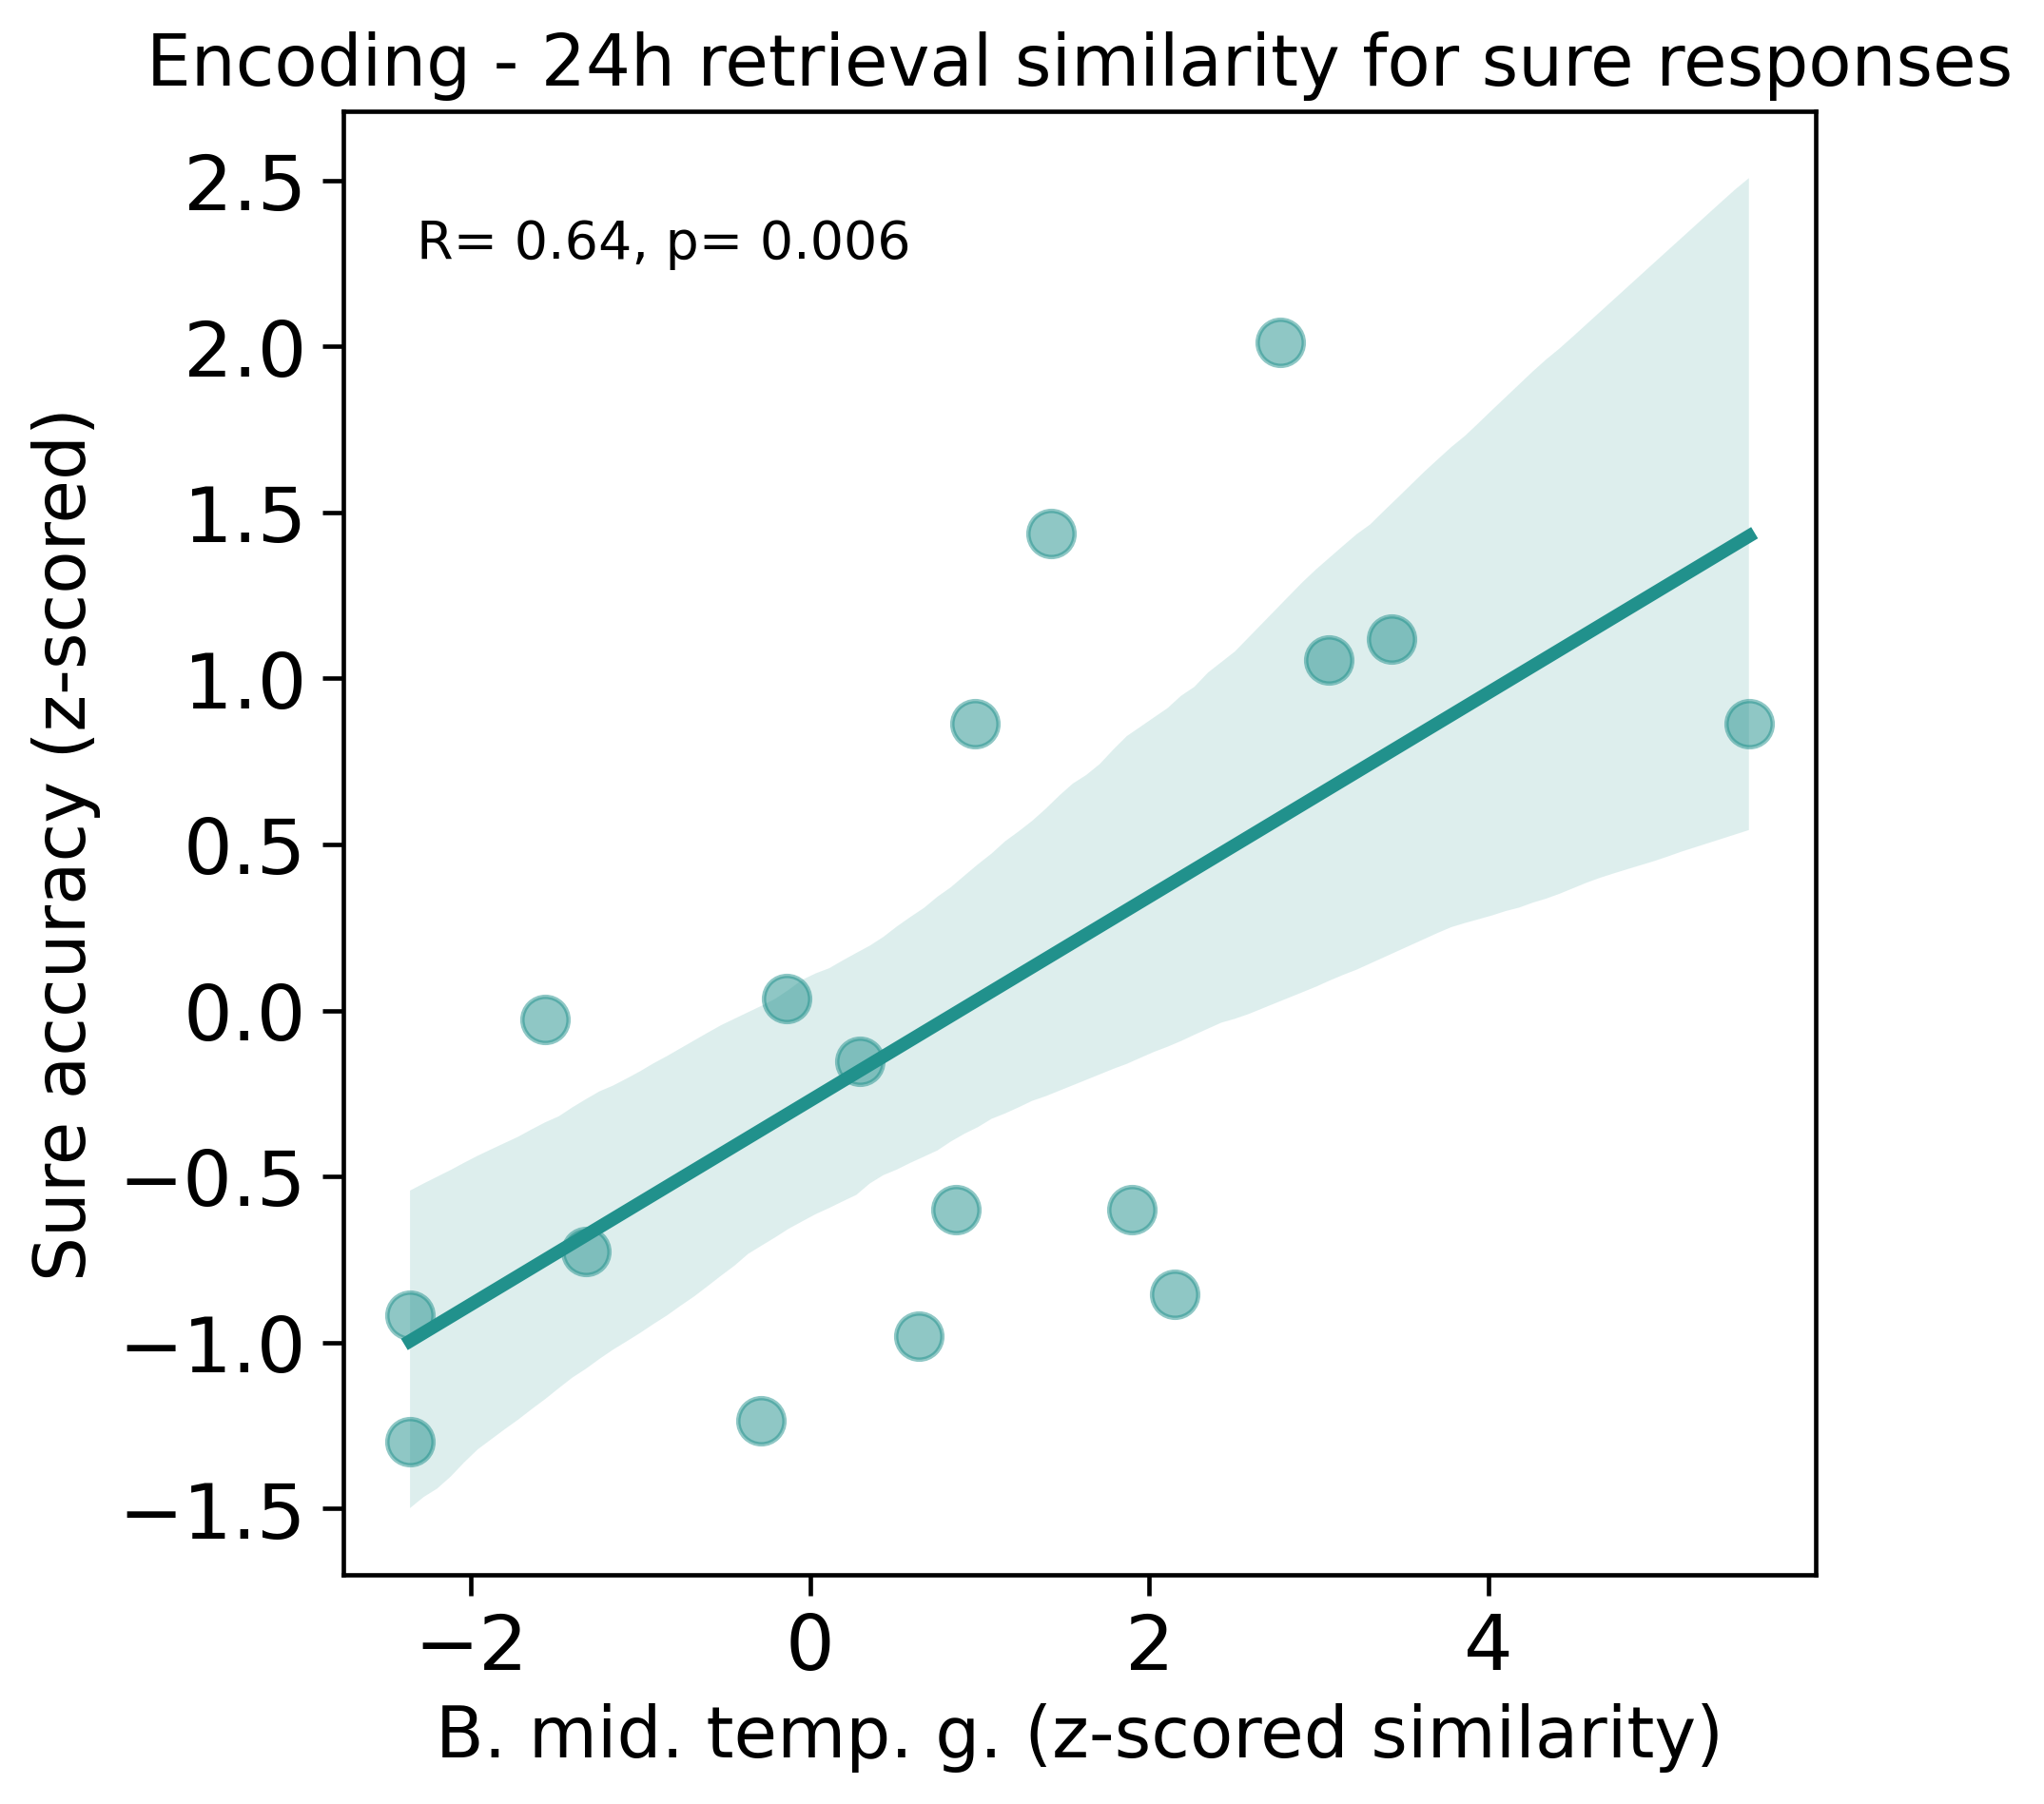
\includegraphics[width=0.6\linewidth]{paper/src/figures/20240530_wb-array_n__enc_ret2_perm_consc_consc-unconsc_incorr_B. mid. temp. g._ERS_correl.png}
     \caption*{\textbf{Figure S3. Similarity of voxel patterns between encoding and the 24-hour category retrieval was relevant for retrieval success.} \\ \vspace{0.5em}
   Encoding - 24-hour category retrieval similarity in bilateral middle temporal gyrus underlying correct sure responses given on the category retrieval task revealed a non-significant mean value comparison but a significant between-subjects correlation with the accuracy of sure responses given on the 24-hour category task (number of correct sure trials, p = 0.006, R = 0.64, B\textsubscript{10} = 10.4). Results presented in this panel were acquired with the whole-brain fMRI sequence. Abbreviations: B., bilateral; mid., middle; temp., temporal; g., gyrus.}
\end{figure}

\newpage

 \begin{figure}[!ht]
    \centering
     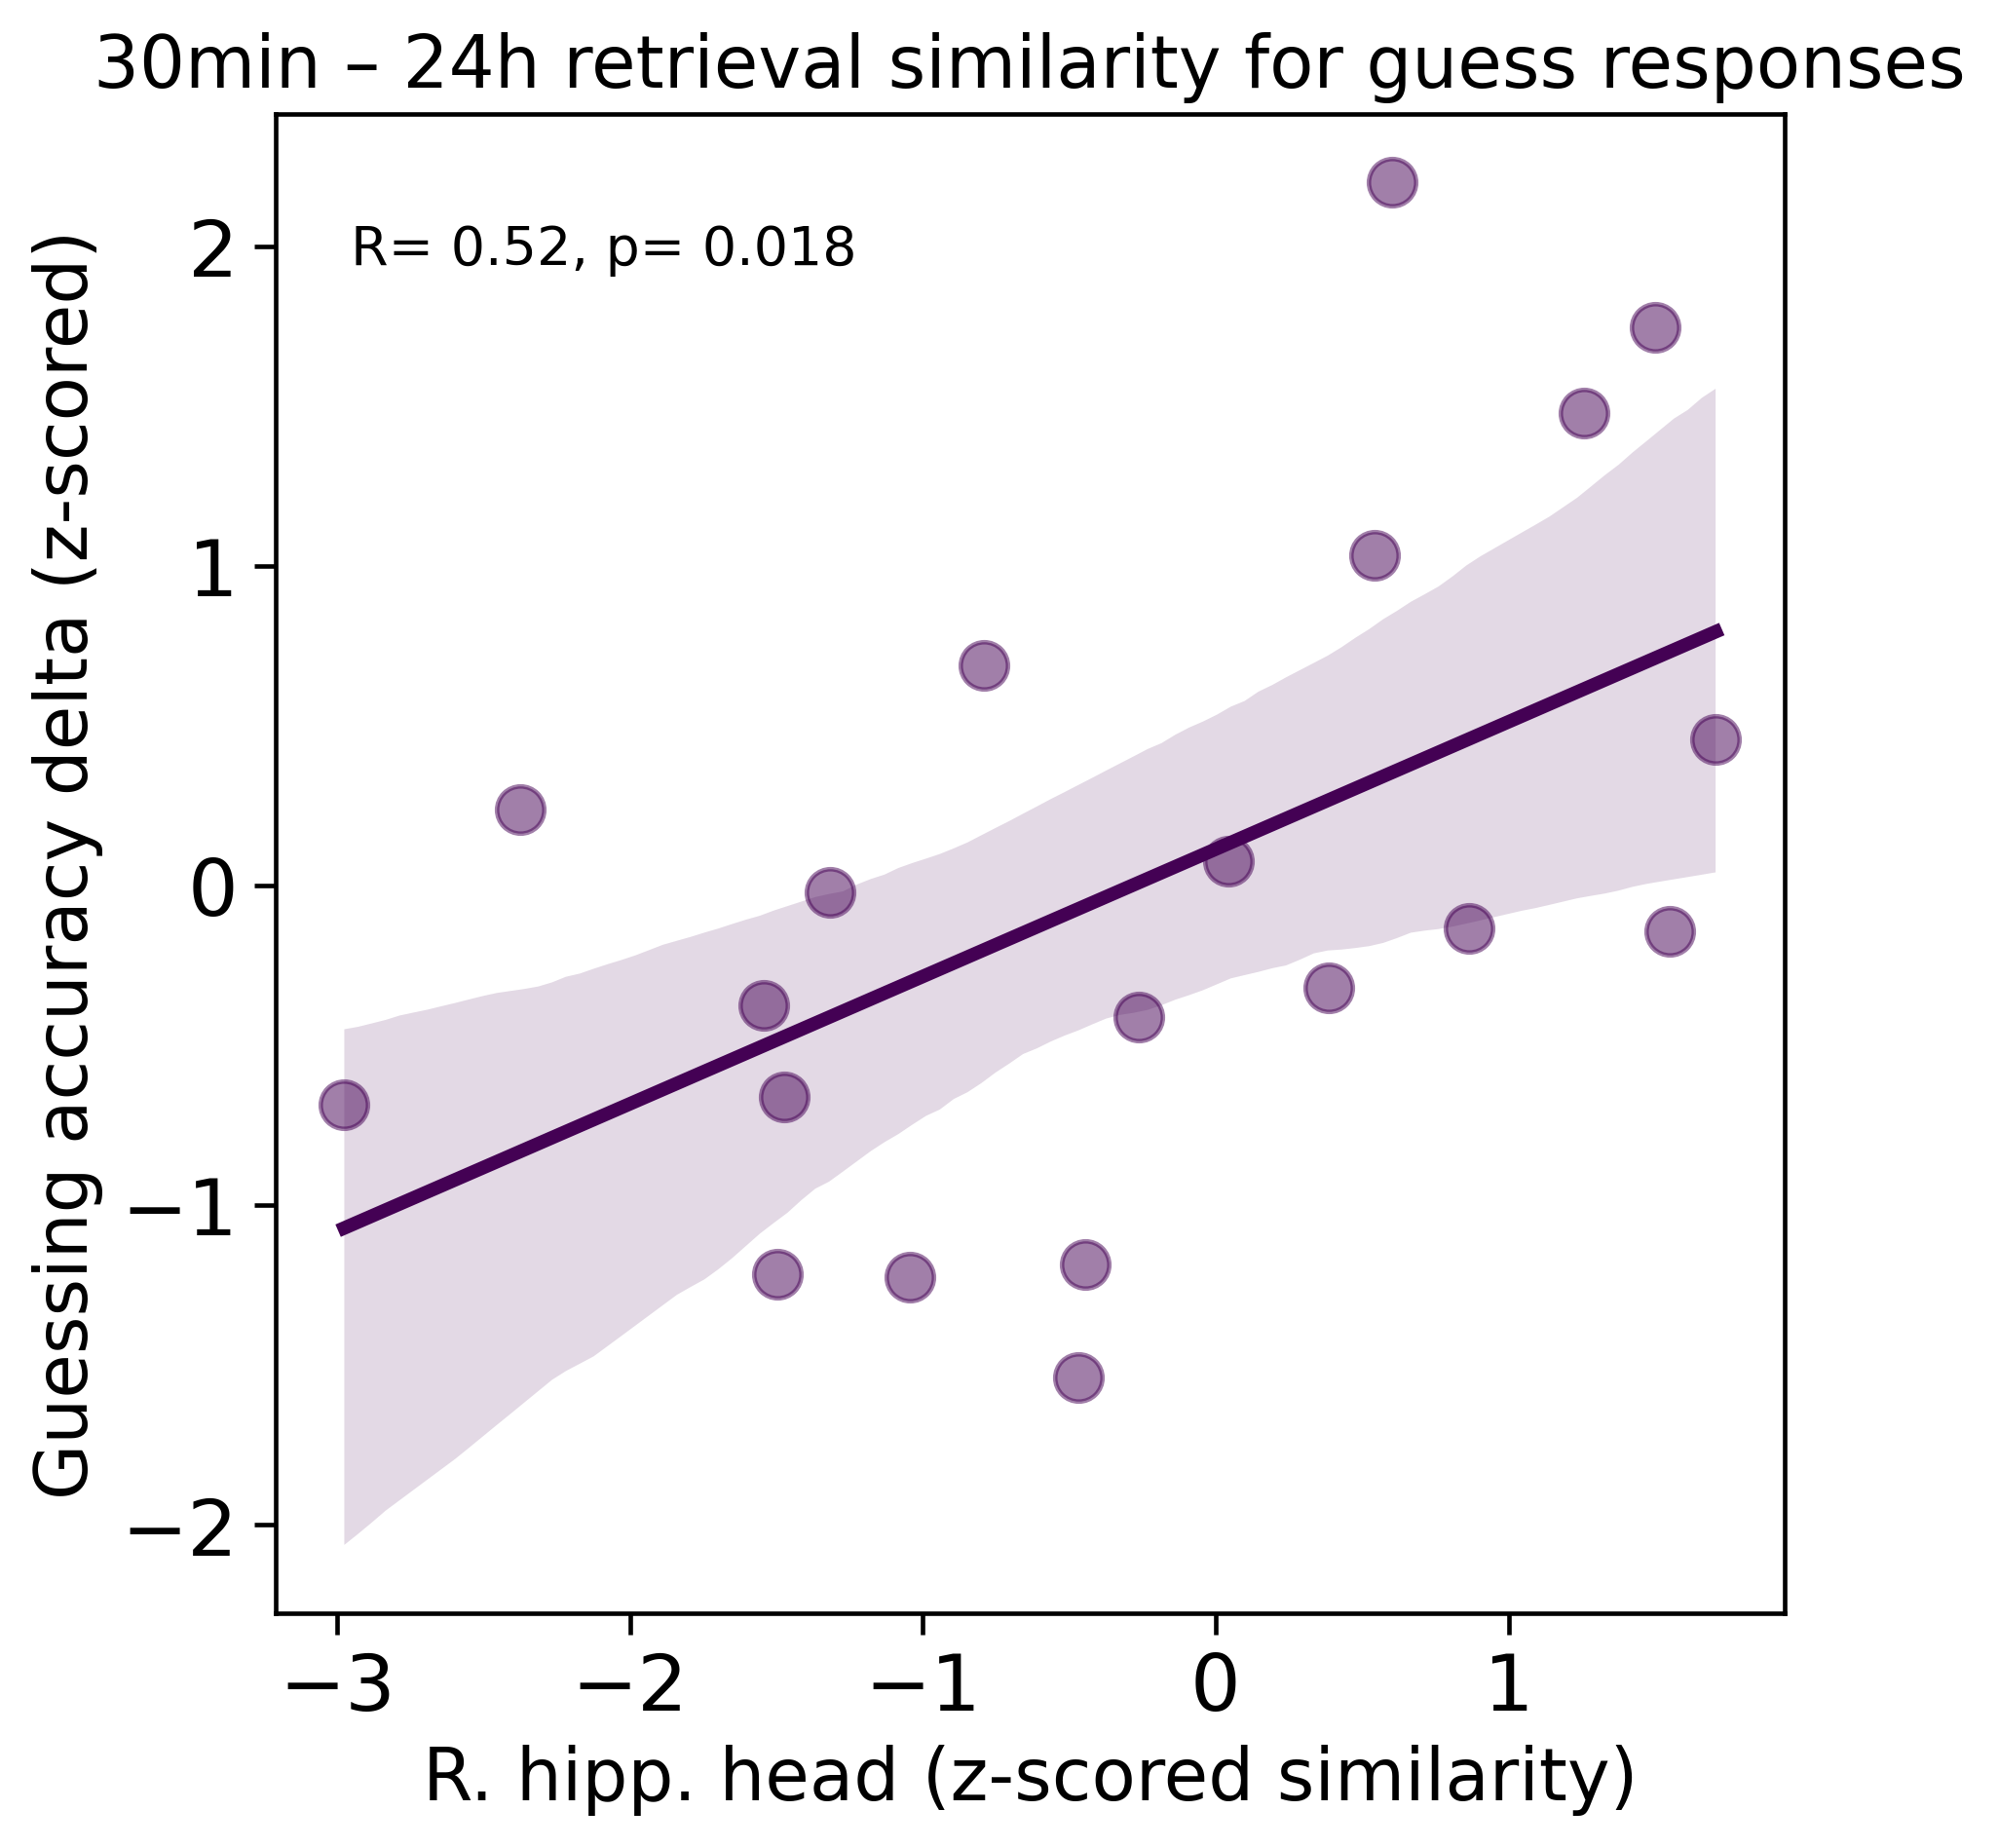
\includegraphics[width=0.6\linewidth]{paper/src/figures/20240530_hipp-array_n_ret1_ret2_perm_consc_unconsc_corr-unconsc_incorr_R. hipp. head_ERS_correl.png}
     \caption*{\textbf{Figure S4. Similarity of voxel patterns between the 30-minute and the 24-hour category retrieval was relevant for the accuracy of guess responses.} \\ \vspace{0.5em}
Retrieval-retrieval similarity of voxel patterns in the right hippocampal head underlying correct guess responses revealed a non-significant mean value comparison but a significant between-subjects correlation with the delta of correct guess responses (i.e., number of correct guess responses at 24 hours minus number of correct guess responses at 30 minutes, p = 0.018, R = 0.52, B\textsubscript{10} = 3.7). Results presented in this panel were acquired with the small FOV fMRI sequence. Abbreviations: R., right; hipp., hippocampus.}
\end{figure}



\newpage

 \begin{figure}[!ht]
    \centering
\begin{subfigure}[]{0.6\linewidth}
    \centering
    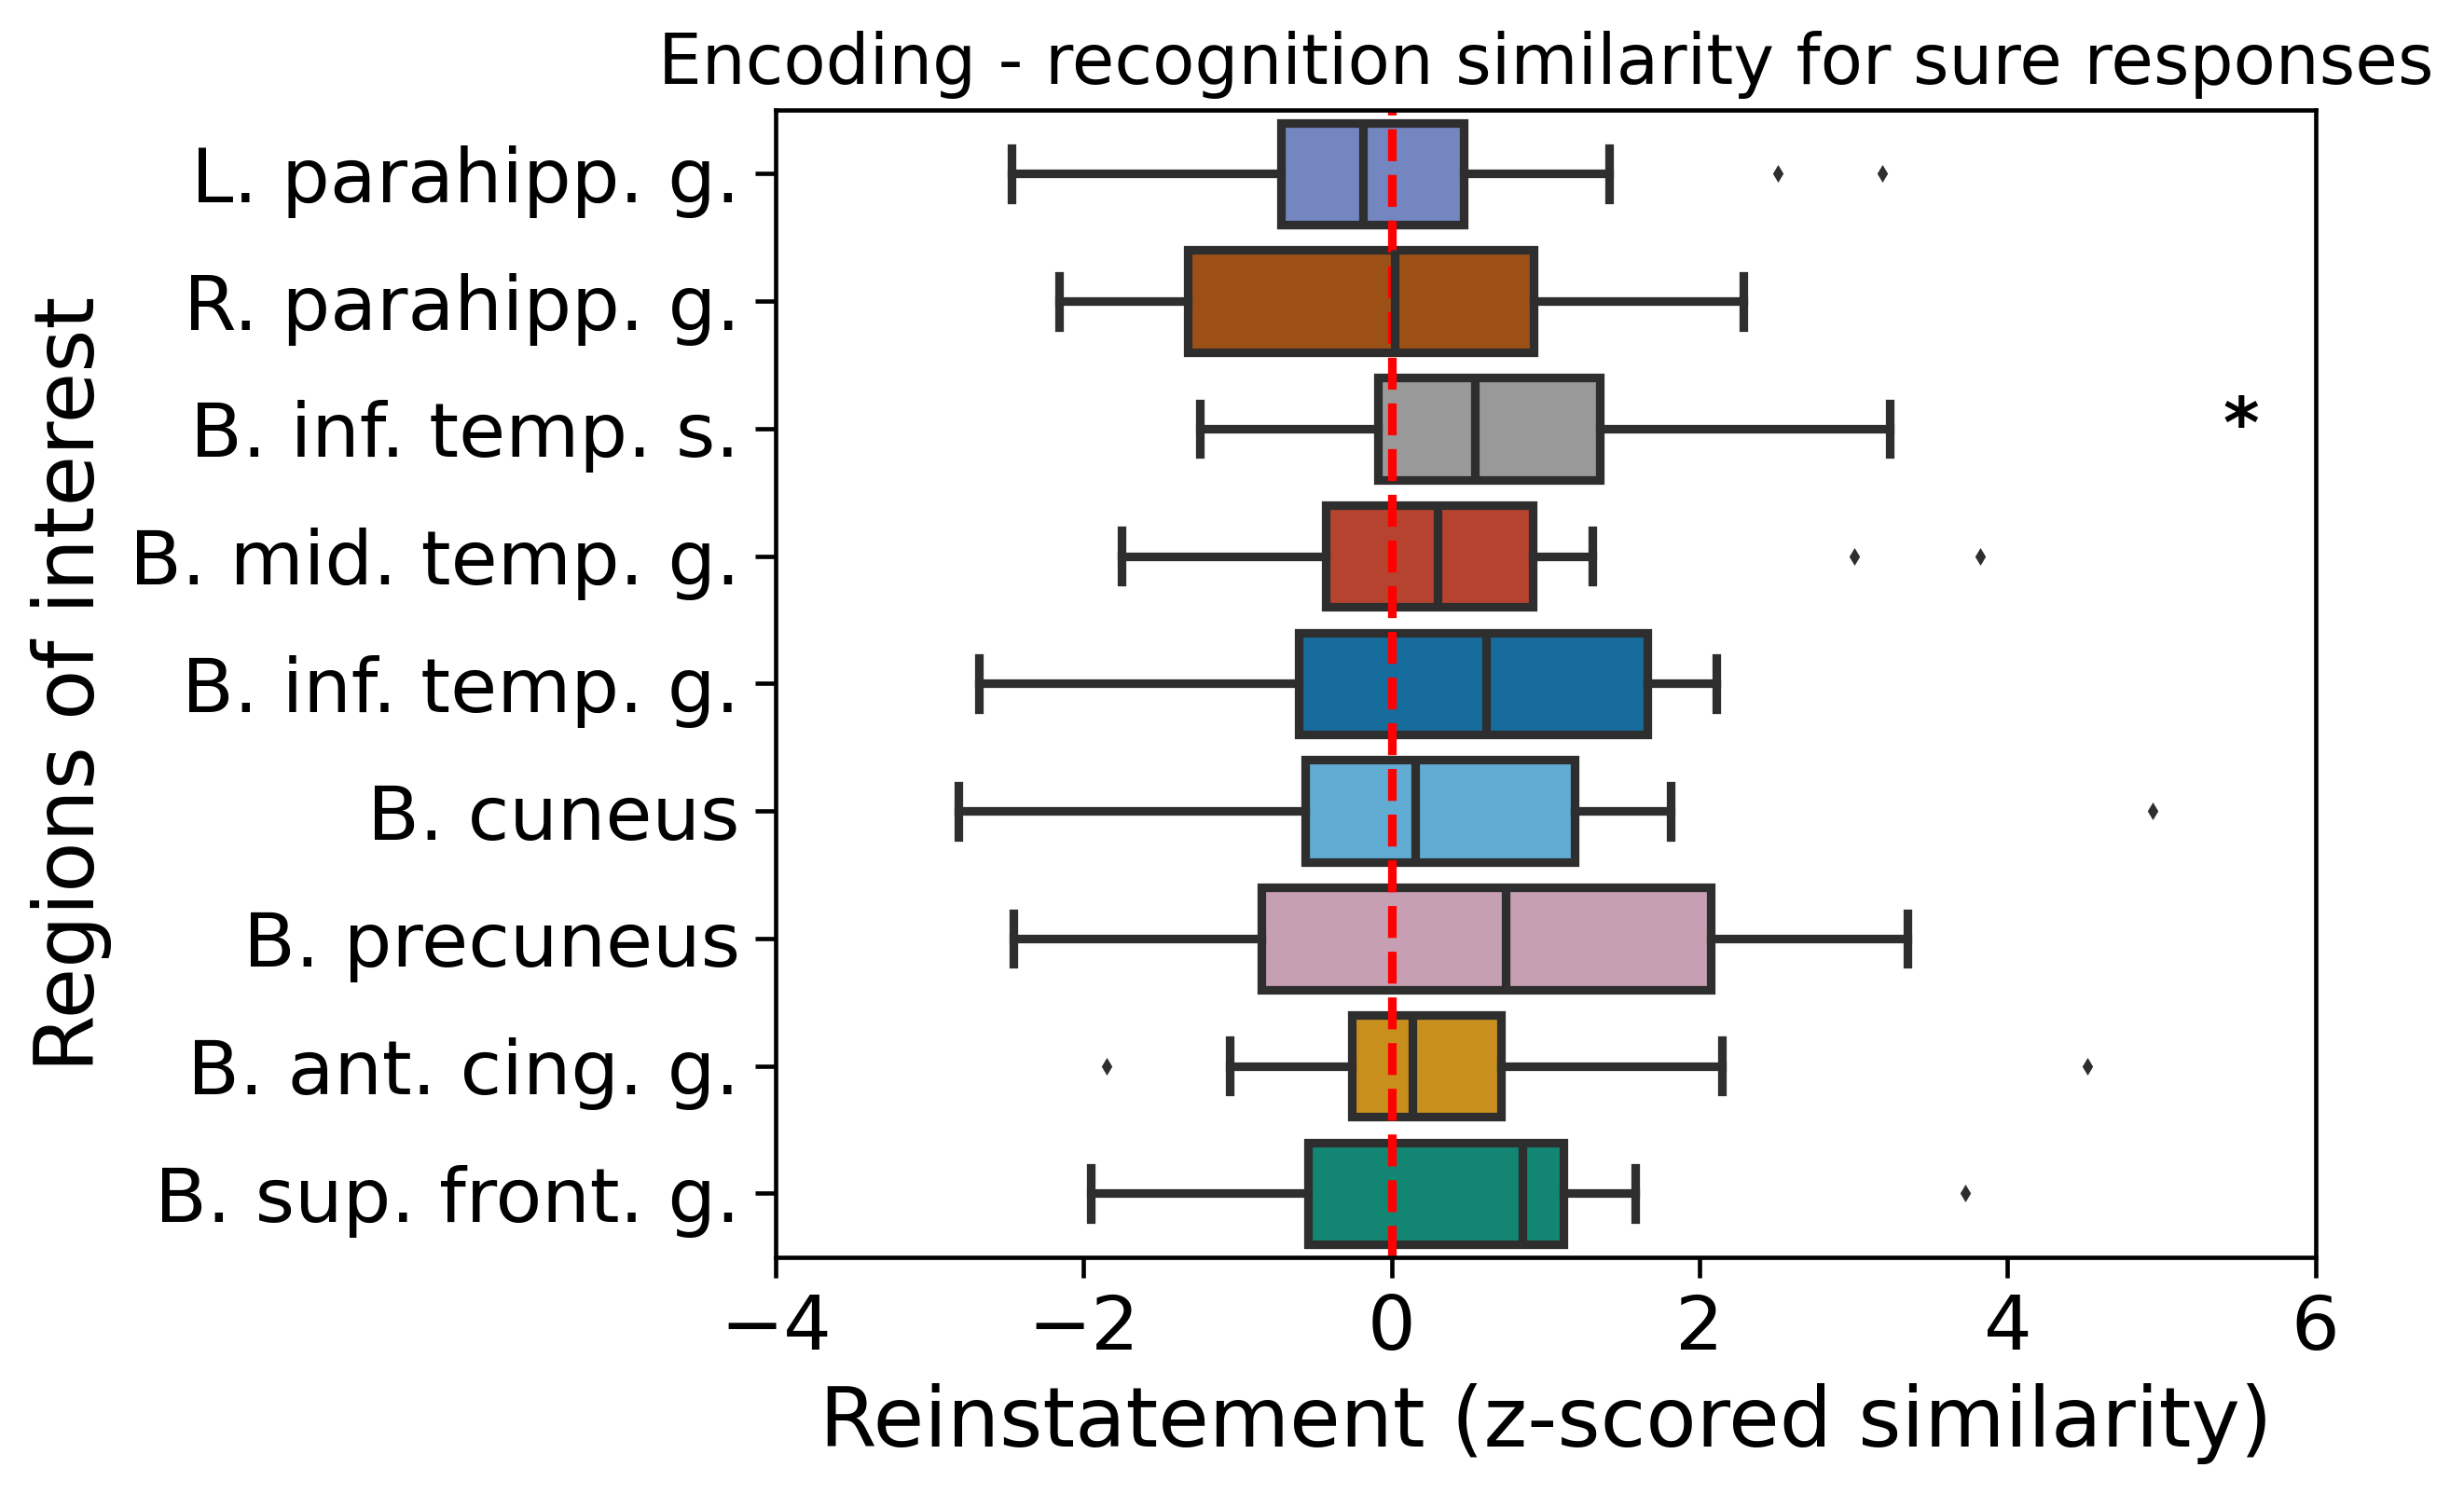
\includegraphics[width=\linewidth]{paper/src/figures/20240710_wb-all_memory_n_enc_recog_perm_consc_consc-unconsc_incorr.png}
\end{subfigure}
\begin{subfigure}[]{0.19\linewidth}
    \centering
    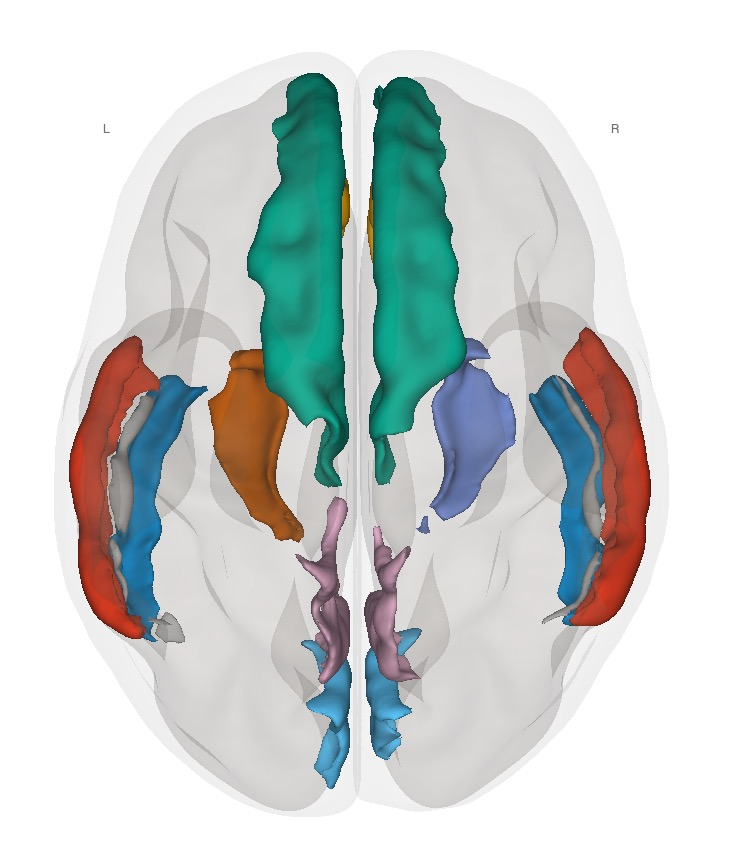
\includegraphics[width=\linewidth]{paper/src/figures/wb_rois_top.jpg}
\end{subfigure}
\begin{subfigure}[]{0.19\linewidth}
    \centering
    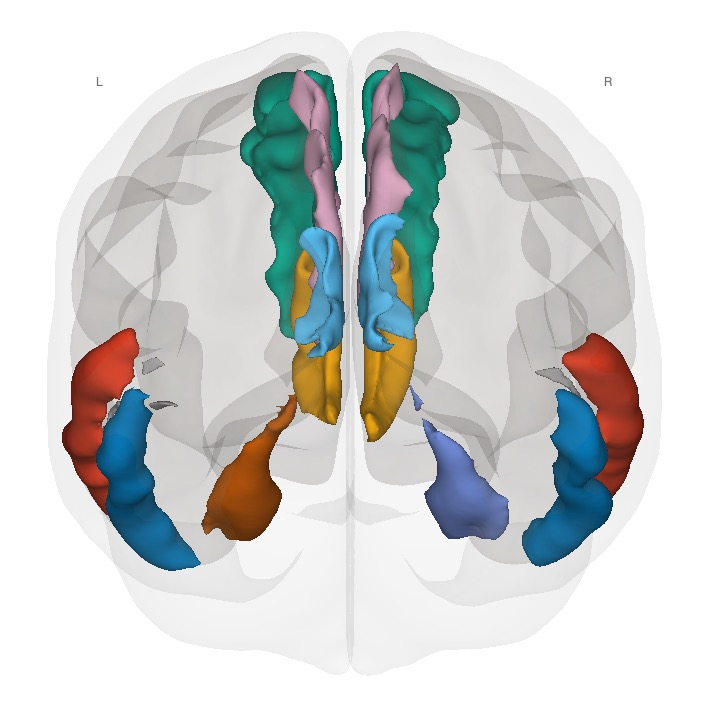
\includegraphics[width=\linewidth]{paper/src/figures/wb_rois_back.jpg}
\end{subfigure}
     \caption*{\textbf{Figure S5. Similarity of voxel patterns between encoding and recognition at 24 hours was relevant for retrieval success.} \\ \vspace{0.5em}
Significant mean value comparison in bilateral inferior temporal sulcus regarding correct sure responses (p = 0.026, t(17) = 2.55, B\textsubscript{10} = 2.9). Results presented in this panel were acquired with the whole-brain fMRI sequence. *p < 0.05, **p < 0.01 by Student’s t test. Abbreviations: R., right; L., left; B., bilateral; parahipp., parahippocampus; inf., inferior; mid., middle; ant., anterior; cing., cingulate; sup., superior; front., frontal; s., sulcus, g., gyrus.
}
\end{figure}


\newpage


 \begin{figure}[!ht]
    \centering
     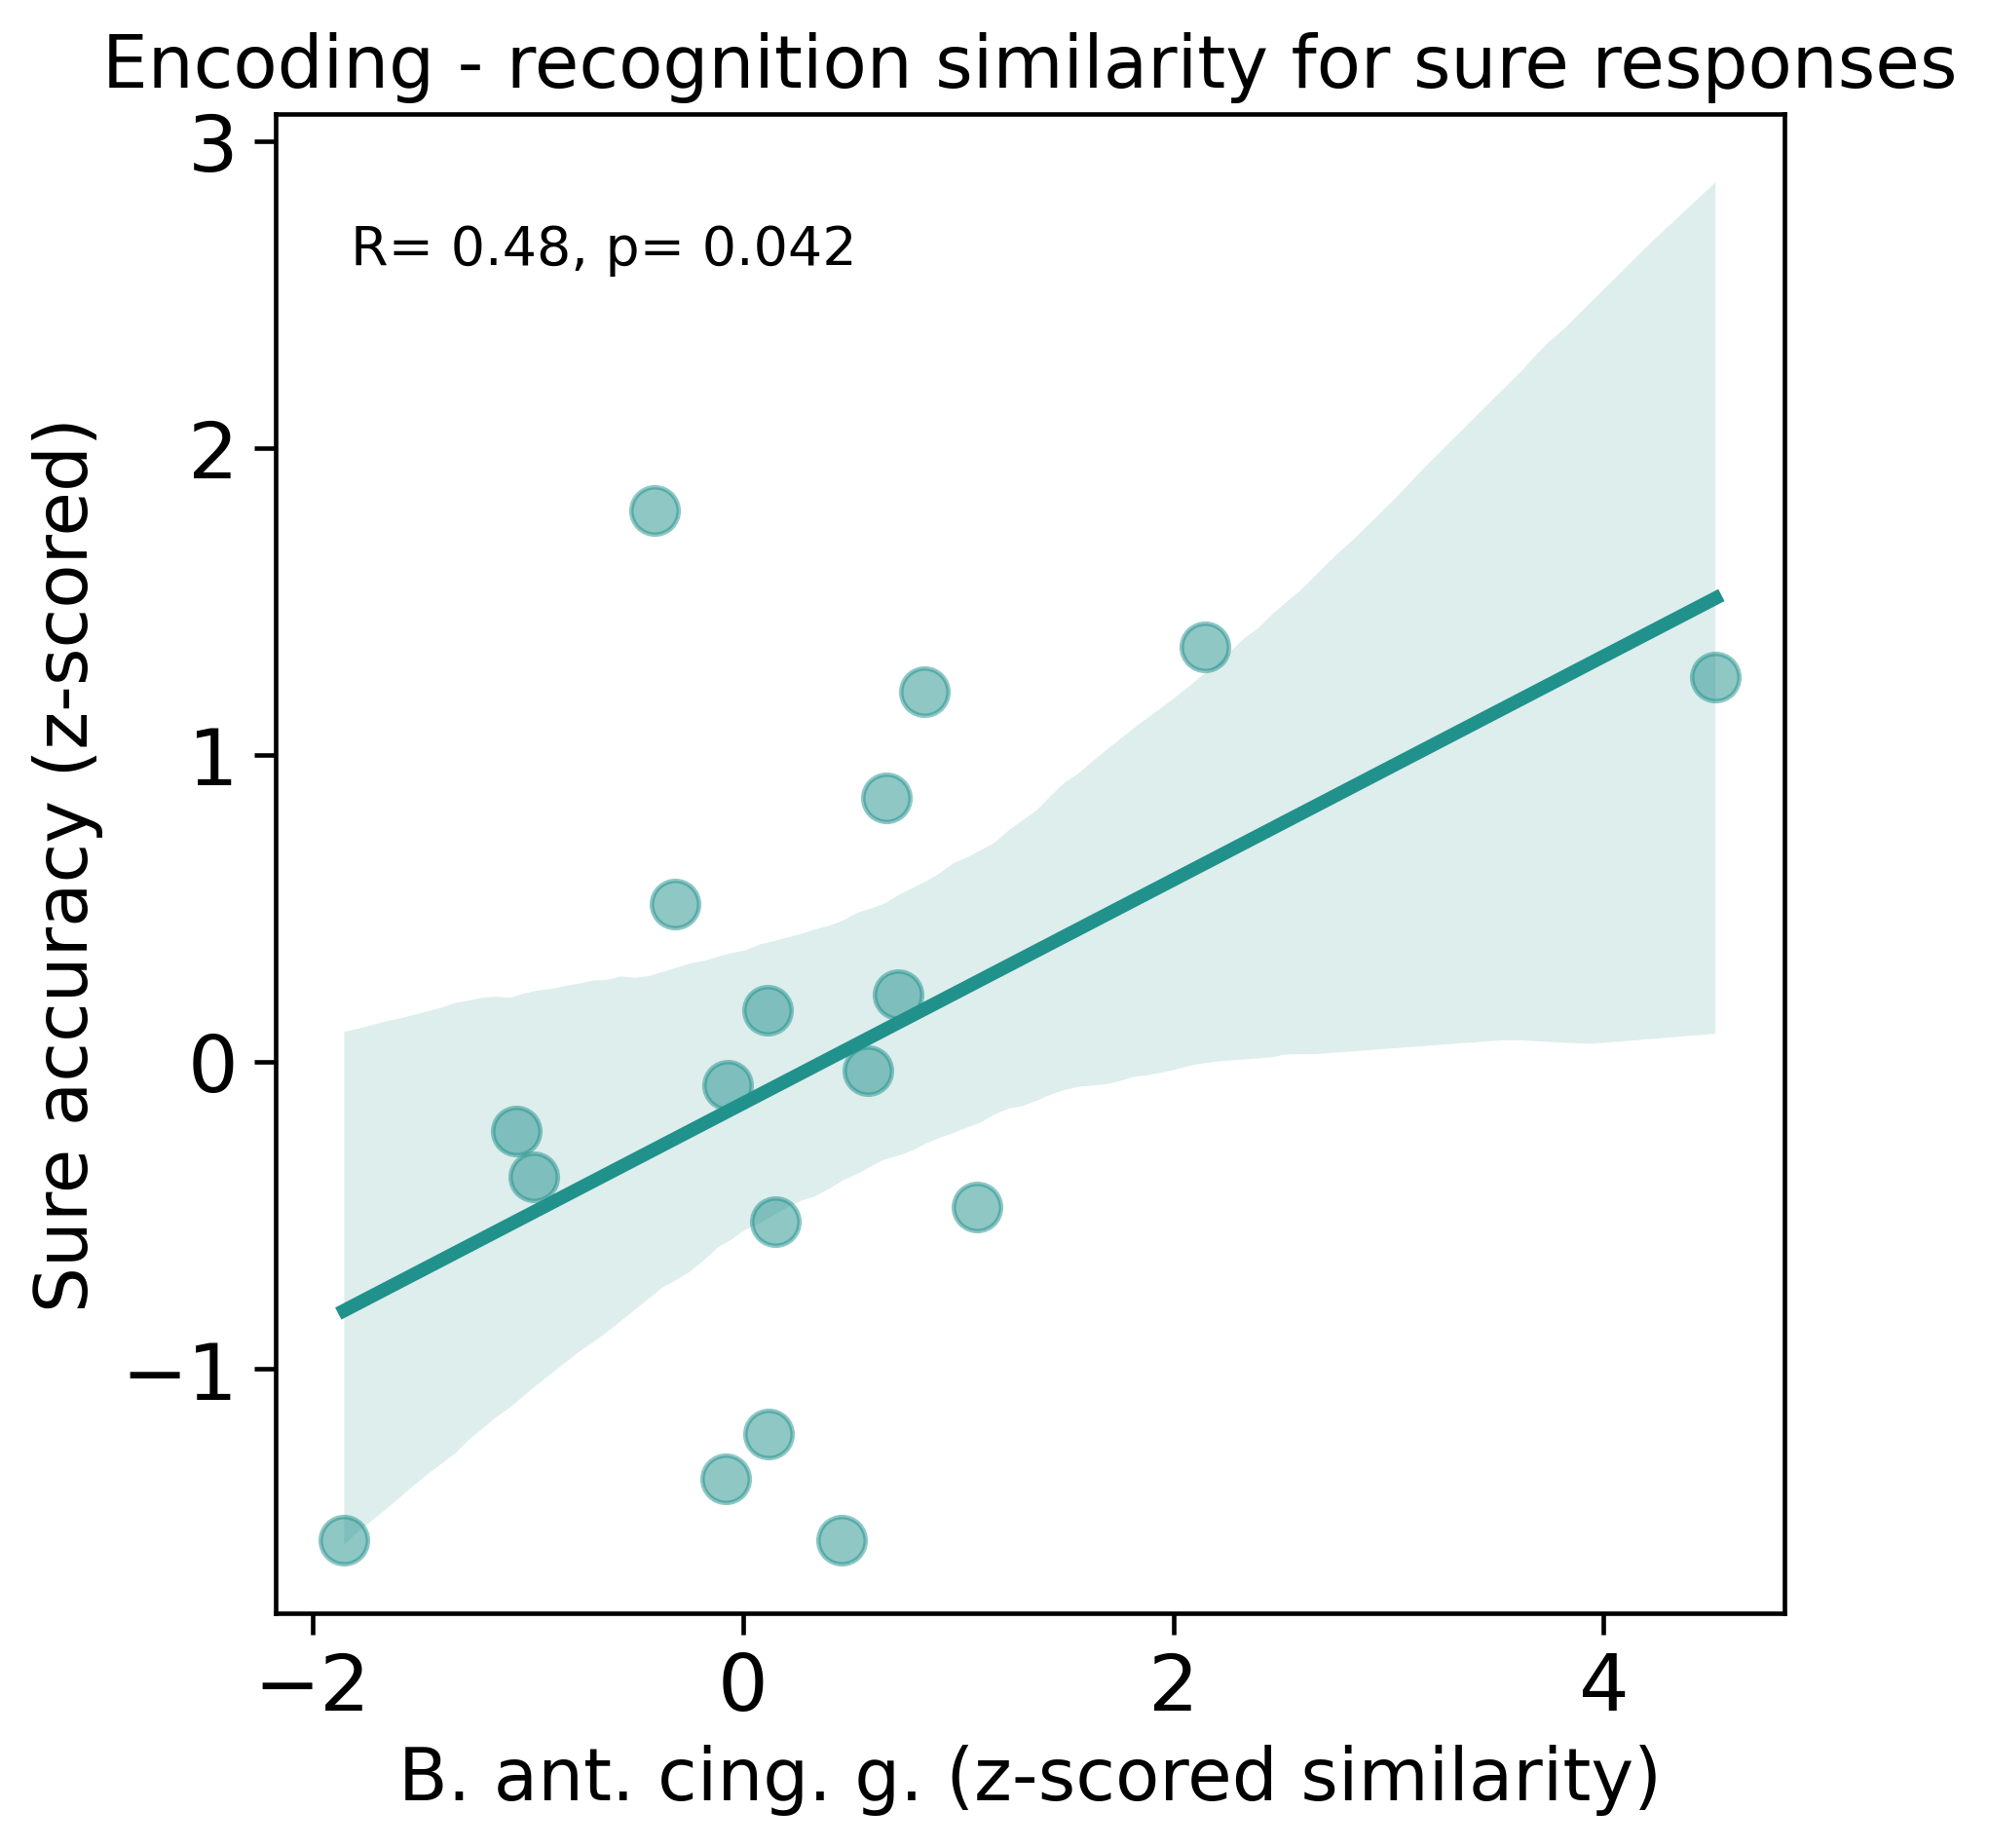
\includegraphics[width=0.6\linewidth]{paper/src/figures/20240710_wb-all_memory_n_enc_recog_perm_consc_consc-unconsc_incorr_B. ant. cing. g._ERS_correl.png}
     \caption*{\textbf{Figure S6. Similarity of voxel patterns between encoding and recognition at 24 hours was relevant for retrieval success.} \\ \vspace{0.5em}
 Pattern similarity in bilateral anterior cingulate gyrus (B. ant. cing. g.) underlying correct sure responses revealed a non-significant mean value comparison but a significant between-subjects correlation with the number of correct sure responses given on the recognition task (p = 0.041, R = 0.48, B\textsubscript{10} = 2.0).  Results presented in this panel were acquired with the small FOV fMRI sequence. Abbreviations: B., bilateral; ant., anterior; cing., cingulate; g., gyrus.}
\end{figure}

